\section{Laboratory work implementation}

\subsection{Tasks and Points}


Basic Level (grade 5 || 6):

-    Create an animation based on Windows timer which involves at least 5 different drawn objects

Normal Level (grade 7 || 8):

-    Realize the tasks from Basic Level.

- 	 Increase and decrease animation speed using mouse wheel/from keyboard

- 	 Solve flicking problem describe in your readme/report the way you had implemented this





\subsection{Laboratory work analysis}
Repository:

https://github.com/StasBizdiga/WP

\subsection{Proving my work}

Basic level: \\

- All the required things are drawn: There are at least 5 different animated objects.

------------------------------------ \\

Normal level: \\

- You can change the animation speed with the mouse wheel. (See instructions below)

- Flickering doesn't seem to occur in my program but regardless, I've had a safe approach. When drawing any of the objects, as the program is about to draw the next frame of the same object, it draws it white first so that it is being erased ,thus we get a smooth, clean of errors animation.


-------------------------------------------------- \\

Hot-keys Instructions:

- Rolling the mouse wheel up accelerates the animation

- Rolling the mouse wheel down decelerates the animation

-------------------------------------------------- \\

Additional Features:

- Animation is ping pong looped. There's a variable that is added to certain parameters, then by the middle animation frame it flips, subtracting, thus returning all back smoothly until the initial state. 
Then the cycle repeats. \\\\\\


The animation:\\

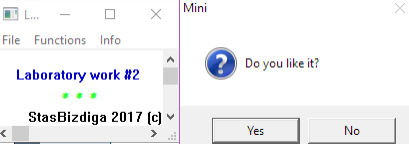
\includegraphics[scale=0.5]{pic_1} \\

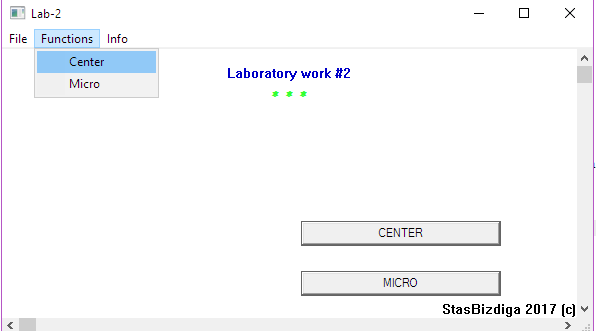
\includegraphics[scale=0.5]{pic_2} \\

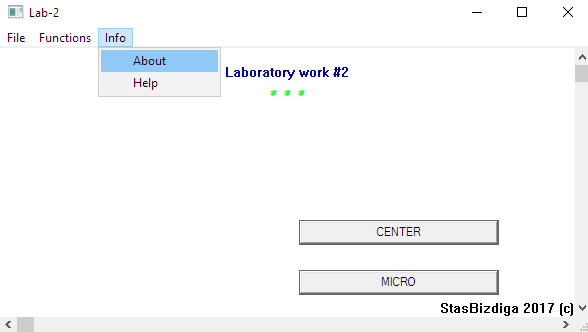
\includegraphics[scale=0.5]{pic_3} \\



\clearpage